% Options for packages loaded elsewhere
\PassOptionsToPackage{unicode}{hyperref}
\PassOptionsToPackage{hyphens}{url}
%
\documentclass[
]{article}
\title{Modeling NFL Fantasy Football Performance}
\author{Ethan Allavarpu}
\date{19 March 2021}

\usepackage{amsmath,amssymb}
\usepackage{lmodern}
\usepackage{iftex}
\ifPDFTeX
  \usepackage[T1]{fontenc}
  \usepackage[utf8]{inputenc}
  \usepackage{textcomp} % provide euro and other symbols
\else % if luatex or xetex
  \usepackage{unicode-math}
  \defaultfontfeatures{Scale=MatchLowercase}
  \defaultfontfeatures[\rmfamily]{Ligatures=TeX,Scale=1}
\fi
% Use upquote if available, for straight quotes in verbatim environments
\IfFileExists{upquote.sty}{\usepackage{upquote}}{}
\IfFileExists{microtype.sty}{% use microtype if available
  \usepackage[]{microtype}
  \UseMicrotypeSet[protrusion]{basicmath} % disable protrusion for tt fonts
}{}
\makeatletter
\@ifundefined{KOMAClassName}{% if non-KOMA class
  \IfFileExists{parskip.sty}{%
    \usepackage{parskip}
  }{% else
    \setlength{\parindent}{0pt}
    \setlength{\parskip}{6pt plus 2pt minus 1pt}}
}{% if KOMA class
  \KOMAoptions{parskip=half}}
\makeatother
\usepackage{xcolor}
\IfFileExists{xurl.sty}{\usepackage{xurl}}{} % add URL line breaks if available
\IfFileExists{bookmark.sty}{\usepackage{bookmark}}{\usepackage{hyperref}}
\hypersetup{
  pdftitle={Modeling NFL Fantasy Football Performance},
  pdfauthor={Ethan Allavarpu},
  hidelinks,
  pdfcreator={LaTeX via pandoc}}
\urlstyle{same} % disable monospaced font for URLs
\usepackage[margin=1in]{geometry}
\usepackage{longtable,booktabs,array}
\usepackage{calc} % for calculating minipage widths
% Correct order of tables after \paragraph or \subparagraph
\usepackage{etoolbox}
\makeatletter
\patchcmd\longtable{\par}{\if@noskipsec\mbox{}\fi\par}{}{}
\makeatother
% Allow footnotes in longtable head/foot
\IfFileExists{footnotehyper.sty}{\usepackage{footnotehyper}}{\usepackage{footnote}}
\makesavenoteenv{longtable}
\usepackage{graphicx}
\makeatletter
\def\maxwidth{\ifdim\Gin@nat@width>\linewidth\linewidth\else\Gin@nat@width\fi}
\def\maxheight{\ifdim\Gin@nat@height>\textheight\textheight\else\Gin@nat@height\fi}
\makeatother
% Scale images if necessary, so that they will not overflow the page
% margins by default, and it is still possible to overwrite the defaults
% using explicit options in \includegraphics[width, height, ...]{}
\setkeys{Gin}{width=\maxwidth,height=\maxheight,keepaspectratio}
% Set default figure placement to htbp
\makeatletter
\def\fps@figure{htbp}
\makeatother
\setlength{\emergencystretch}{3em} % prevent overfull lines
\providecommand{\tightlist}{%
  \setlength{\itemsep}{0pt}\setlength{\parskip}{0pt}}
\setcounter{secnumdepth}{-\maxdimen} % remove section numbering
\ifLuaTeX
  \usepackage{selnolig}  % disable illegal ligatures
\fi

\begin{document}
\maketitle

{
\setcounter{tocdepth}{1}
\tableofcontents
}
\vfill

\hypertarget{abstract}{%
\section{Abstract}\label{abstract}}

In this paper, I plan to discuss two main aspects of drafting a fantasy
football team. In the first section, I consider the variability present
within starter-quality players for each of the main offensive
positions--quarterback (QB), running back (RB), wide receiver (WR), and
tight end (TE)--to determine if there is an inherent strategy at play
regarding which position to prioritize. In the second portion, I develop
a predictive model to decide a player's potential success regarding
fantasy football points based on his statistics from the prior year. For
both the analysis and the models, I consider fantasy football leagues
that utilize ESPN PPR (point per reception) scoring rules in a 12-team
format with the following offensive lineup: 1 QB, 2 RB, 2 WR, 1 TE, and
1 flex position, which can be an additional RB, WR, or TE. In this
paper, though, I will omit the influence of the flex position to
consider the four positions independently for model building.

\newpage

\hypertarget{introduction}{%
\section{Introduction}\label{introduction}}

Fantasy football captivates many sports fans each season. Whether it is
daily fantasy or a season-long commitment, managers search for the best
players to acquire for their teams in the upcoming NFL season. A variety
of different scoring methods exist--from standard to PPR to custom
scoring methodologies. While this analysis can be easily adapted to any
scoring system, I will limit it to PPR scoring since this tends to be
the most common form seen across platforms.

PPR scoring\footnote{PPR scoring:
  \url{https://support.espn.com/hc/en-us/articles/360031085331-League-Scoring-Types-Standard-and-PPR}}
is an add-on scoring system to the standard scoring system\footnote{Standard
  scoring:
  \url{https://www.espn.com/fantasy/football/ffl/story?page=fflrulesstandardscoring}}
with the singular difference being that players receive an additional
point for each reception made throughout the season, placing additional
weight on the RB, TE, and WR positions.

\hypertarget{data-collection}{%
\section{Data Collection}\label{data-collection}}

I took most of my data from Pro Football Reference\footnote{Pro Football
  Reference: \url{https://www.pro-football-reference.com/}}. I gathered
.csv files on the performance of NFL players--including statistics as
well as fantasy points scored--from the 2010 to 2020 NFL seasons. I
chose the 11 most recent seasons because football continuously evolves
season after season, so the most recent seasons will look the most
similar to the 2021 NFL season, for which I am trying to predict player
success. Even 11 seasons is a bit of a stretch--the game in 2019 looked
markedly different from that in 2012, but I required the 10 data
groupings from 11 seasons due to a need for adequate sample sizes.

To decide a cutoff for players to include in my analysis, I utilized the
influence of the starting lineup slots as defined in the abstract (1 QB,
2 RB, 2 WR, 1 TE, 1 flex). Now, the flex position is a bit variable
(i.e., managers often use bench players with the best matchup), so for
determining which players to use, I ignored the influence of the flex
spot. This led me to include one player for each opening on a roster,
plus an additional player for each position in a bench role. So, when
accounting for a 12-team league, I limited the players in my data set to
players with the following position rank (i.e., their PPR score rank
among players at the same position) in the prior season: top 24 (12 +
12) for QB and TE, and top 36 (24 + 12) for RB and WR. This cutoff
existed for both \emph{next year's scores} and \emph{this year's data}
to remove players that may have been injured or ``fell off a cliff''
(i.e., dropped drastically in production): such players would be
outliers that would skew my predictions.

While parsing through the data, I encountered a few edge cases which I
had to address. Some players had the same name, making player-matching a
little difficult. For this analysis, I only included the ``best'' player
with a given name, as it is improbable that there are two high-end
players with the same name.

Additionally, some features had \texttt{NA} values for a few
observations, which I addressed based on context:

\begin{itemize}
\tightlist
\item
  For rush yards per attempt (YPA) and receiving yards per catch (YPC),
  the \texttt{NA} values likely resulted from
  \(\frac{0 \text{ yards}}{0 \text{ attempts}}\) or
  \(\frac{0 \text{ yards}}{0 \text{ catches}}\), respectively; for my
  analyses, I set these instances to 0.
\item
  For \texttt{two\_pt\_made}, \texttt{two\_pt\_pass}, and
  \texttt{fmb\_lst} (i.e., two-point conversions (rush/receive),
  two-point conversions (pass), and fumbles lost), \texttt{NA} values
  likely result from 0 two-point attempts or 0 fumbles, respectively, so
  it would be useless to add values in these observations. Therefore, I
  have chosen to assign a value of 0 to the instances of \texttt{NA} for
  these two variables.
\item
  VBD and the overall rank for some players is \texttt{NA}. However,
  these statistics are calculated using standard scoring, \emph{not}
  PPR; therefore, for my analysis, I have chosen to remove these two
  features for subsequent analyses.
\end{itemize}

\newpage

\hypertarget{variability-by-positions}{%
\section{Variability by Positions}\label{variability-by-positions}}

After cleaning the data appropriately, I wished to look at the
variability by position to determine if there is a position which
managers should draft first in their leagues. While my second section
will help to determine the best players at each position, this part
serves to tell us if there is a certain position that should be drafted
before the others. In a draft, managers have to prioritize which
positions to fill first when constructing their rosters, so finding the
most variable positions can tell us which positions have the largest
drop in performance.

Most managers follow the tenet that they should draft running backs and
wide receivers earlier than quarterbacks and tight ends because those
two positions are perceived as the ``most volatile'' (i.e., they have
the greatest variance in scores for a given season). Therefore, I have
included this section to determine if there is any merit to this belief.
Before conducting significance tests, though, I first wanted to
visualize the data to see if there were any interesting patterns
regarding the spread of the data.

\begin{center}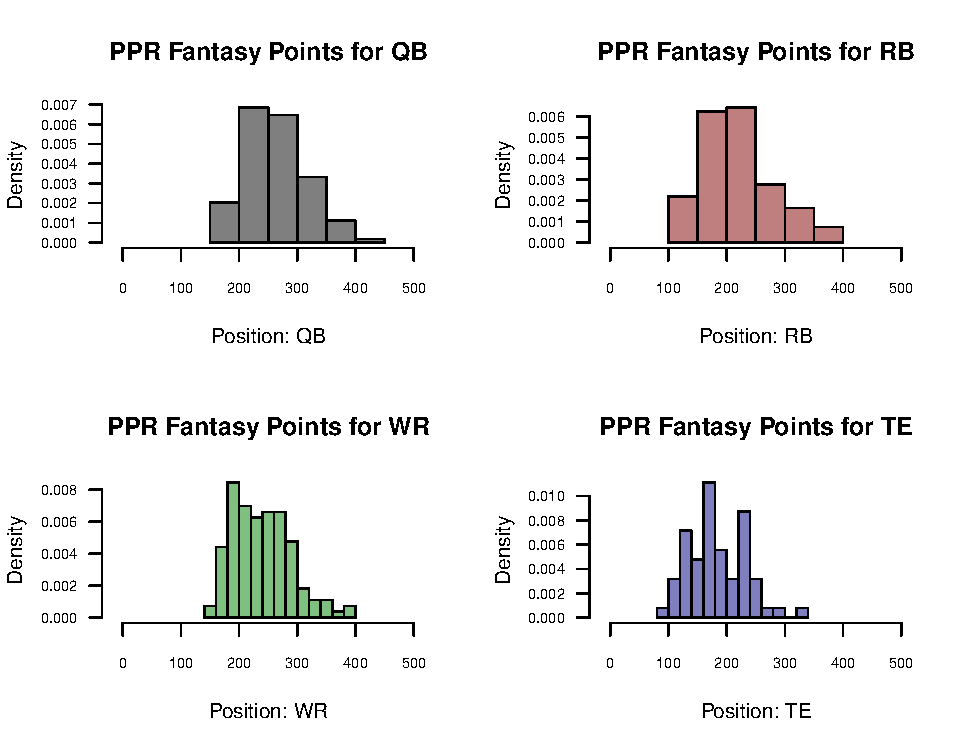
\includegraphics[width=0.85\linewidth]{stats_199_final_report_files/figure-latex/unnamed-chunk-1-1} \end{center}

The above histograms demonstrate the right-skewed nature of PPR scores.
Most players will hover around a central point, with a few elite players
pushing the boundary and truly separating themselves from the pack.
While I can see that--since the x-axis of each histogram is on the same
scale--the difference in the spread does not seem too drastic between
positions, I will need further investigation, which is why I chose to
incorporate side-by-side boxplots as well.

\begin{center}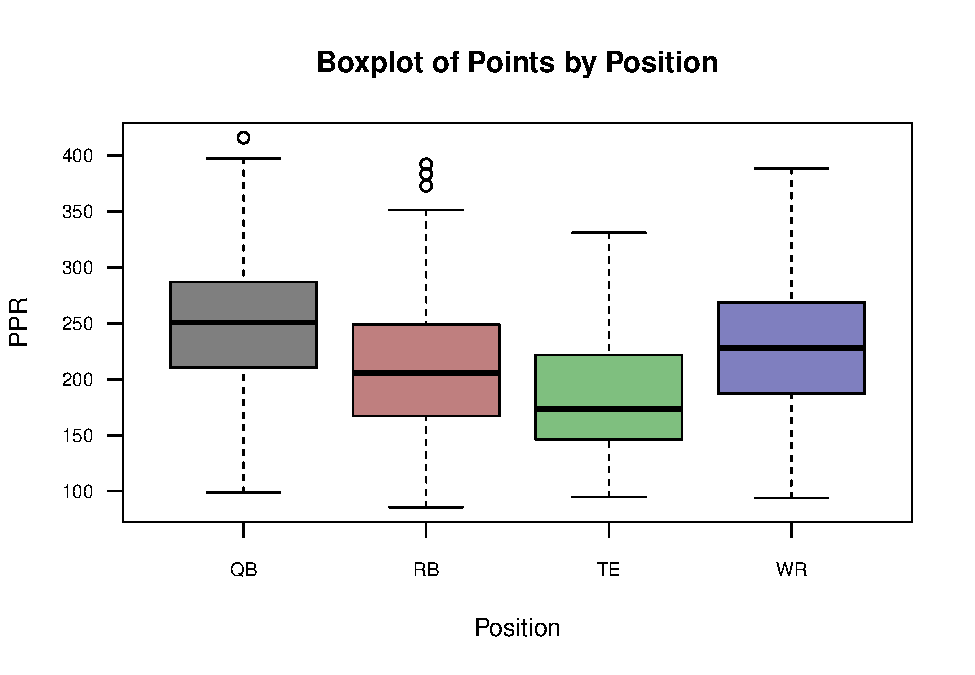
\includegraphics[width=0.85\linewidth]{stats_199_final_report_files/figure-latex/unnamed-chunk-2-1} \end{center}

\begin{longtable}[]{@{}lrrrr@{}}
\caption{PPR Quartiles by Position}\tabularnewline
\toprule
& QB & RB & TE & WR \\
\midrule
\endfirsthead
\toprule
& QB & RB & TE & WR \\
\midrule
\endhead
Q1 & 210.5 & 167.00 & 146.1 & 187.3 \\
Q3 & 287.0 & 249.15 & 221.8 & 268.8 \\
IQR & 76.5 & 82.15 & 75.7 & 81.4 \\
\bottomrule
\end{longtable}

The boxplots above seem to agree with the histograms. While the range
for each position seems different (in particular, the TE position seems
to have a smaller range than the others), the interquartile ranges are
all roughly equal, seeming to suggest that no position should take
precedence over the others. To confirm these findings, I will consider
using Levene's test to test for equal variance.

\begin{longtable}[]{@{}lrrr@{}}
\caption{Levene's Test for Homogeneity of Variance}\tabularnewline
\toprule
& Df & F value & Pr(\textgreater F) \\
\midrule
\endfirsthead
\toprule
& Df & F value & Pr(\textgreater F) \\
\midrule
\endhead
group & 3 & 2.008 & 0.1117 \\
& 598 & NA & NA \\
\bottomrule
\end{longtable}

The p-value for Levene's test is 0.1117; since this is greater than the
standard significance threshold of \(\alpha = 0.05\), I fail to reject
the null hypothesis. Therefore, I do not have evidence of different
variances between the groups, suggesting that, when filling out my
roster, I should go by the projected fantasy points alone (until a
position is filled) rather than placing preference on certain positions
(as many managers traditionally do with RB and WR). This is not the only
viable draft strategy, though; one other method could be to see which
player has the largest difference over the next best available player at
a given position (since the variability could very well be the same
across all four groups). Again, the purpose of this part of my paper was
to show a difference (or lack thereof) in the variances of the four
positions, \emph{not} to promote or support a specific draft mindset.

\newpage

\hypertarget{predicting-future-results}{%
\section{Predicting Future Results}\label{predicting-future-results}}

\hypertarget{constructing-the-models}{%
\subsection{Constructing the Models}\label{constructing-the-models}}

To predict next season's fantasy success for each player, I divided my
data set into four categories by position (QB, RB, WR, TE), developing a
separate model for each. In each instance, I created a training set and
a validation set by randomly selecting three years (out of ten) to be
combined into a single validation set, while the other seven were
treated as my training set. After developing the best model for each
position, I used it to predict next year's fantasy football points for
each player in my test data set.

When predicting future fantasy football success, I ran into a minor
limitation at the start of my model construction: a lack of variables.
To address this issue, I created a few variables that I believed would
display weekly success, such as passing, rushing, and receiving yards
\emph{per game} for each position. I added these variables to help
demonstrate high-quality production each week to complement the
consistency shown by cumulative yearly totals. In addition to these
elements, I incorporated a completion percentage variable
(\(\frac{\text{completions}}{\text{attempts}}\)) for the quarterback
that demonstrates how accurate a quarterback was during a given season.
After incorporating these additional transformations, I considered my
background in football. Inherently, players tend to cluster together
into tiers depending on ability (e.g., elite, good, average) and play
style (run-first, pass-first). Therefore, to account for these
differences--and thus create a model that has slightly different weights
for each group--I performed K-means clustering to divide the training
set into clusters. I did not have a specific number of clusters in mind;
rather, I performed clustering using 2 to 25 clusters and made a
judgment regarding when the between-cluster sum of squares ``leveled
off'' (i.e., there was not a drastic improvement after adding another
cluster).

After adding the additional variables and features, I constructed a
variety of models for predictions, using validation mean-squared error
(MSE) in conjunction with plots comparing the validation set predictions
to the validation observed values--essentially a residual plot, but for
the validation set instead of the training set--to search for the model
which provides the best accuracy\footnote{While the lowest MSE is ideal,
  there are a few instances in which I pick a model that does \emph{not}
  have the lowest MSE. I did this because, as will be explained later,
  sometimes it is better to have a slightly worse MSE if the model more
  than offsets the worse MSE with an increase in interpretability and
  simplicity.}. Throughout the process, I considered both different
models as well as different transformations: I looked at simple linear
regression, multivariate linear regression, bagging models, ridge
regression, LASSO, and SVM (support vector machines) for regression to
see the best model. I also considered log transformations of both the
predictor as well as response variables to better fit a potential
non-linear relationship.

One thing I considered at the outset was if my model could perform
better than a traditional default of predicting next year's fantasy
football points purely on this year's; this was the first model I
constructed as my ``simple linear model'': univariate and likely how
most people would consider picking certain players. As explained below,
the models constructed for each position had varying degrees of
complexity and interpretability; some were close to the basic linear
model I mentioned, others were too complicated for simple inference on
the predictor variables.

Before I delve into the final candidate model for each respective
position, I would like to acknowledge the difficulty in predicting
sports statistics (of which fantasy football scores are an extension)
due to the random factors in sports. While sports analytics have come a
long way in terms of predictive accuracy, it is the unpredictable which
makes sports fascinating to watch and keeps viewers and fans
entertained.

\hypertarget{final-models}{%
\subsection{Final Models}\label{final-models}}

\hypertarget{qb}{%
\subsubsection{QB}\label{qb}}

For the quarterback position, the best model in terms of MSE was the
multivariate linear model (MSE of 2657.062), but I chose to use a LASSO
model (MSE of 2879.755) after a log transformation on the response
variable. The reason for my decision is that while the linear model
performed better on the validation data, I was worried that including
too many variables in a model, especially when the model is additive,
could lead to overfitting; in turn, this would make my model too
dependent on the specific data I had.

\begin{center}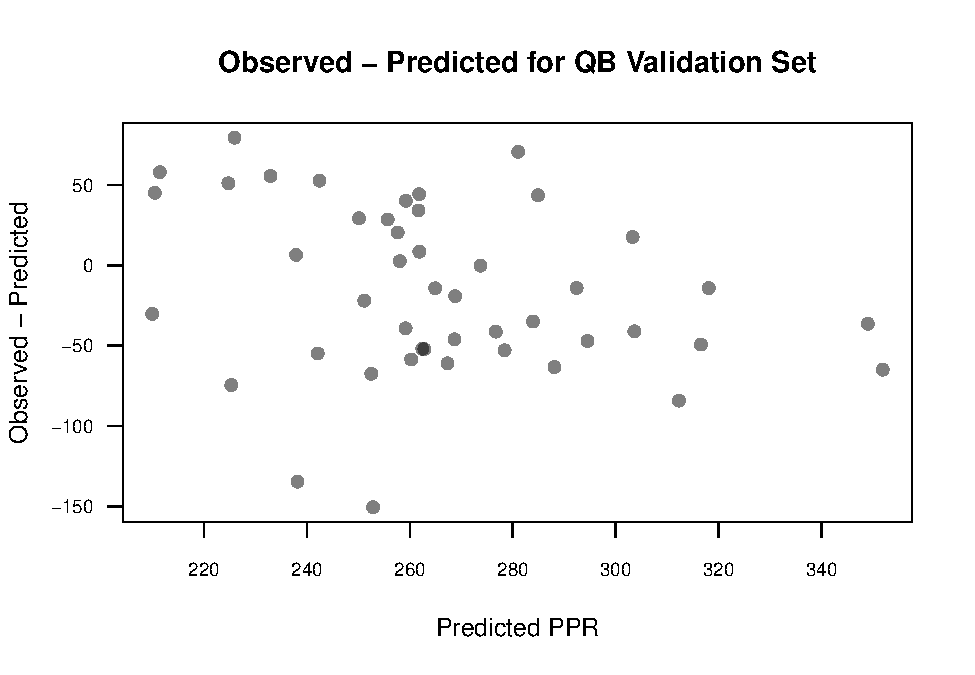
\includegraphics[width=0.85\linewidth]{stats_199_final_report_files/figure-latex/unnamed-chunk-5-1} \end{center}

Based on the above plot, it seems like there might be a slight trend in
my validation predictions which indicates that I may potentially be
missing variable in my model, but on the whole, the plot seems alright
(and thus generally valid and useful for predictions). With this final
model, therefore, the only included variables are pass yards and the
prior year's PPR score:

\[
\hat{\log(y)}= \ensuremath{3.9638\times 10^{-5}}(\text{pass yards}) + 0.0017(\text{PPR})
\] \[
\hat{y}= e^{\ensuremath{3.9638\times 10^{-5}}(\text{pass yards}) + 0.0017(\text{PPR})}
\]

From this model, we can see that, realistically, only two main factors
need to be considered for next year's predictions for quarterbacks:
their passing yardage total and how many PPR points they scored last
year. While these two predictors are not independent (PPR is a linear
combination of a variety of other variables), we see that we don't need
much more than the basic statistics for a quarterback to predict his
future success.

Contextually, quarterbacks do not receive as many points for a touchdown
pass (4) as running backs and receivers do for a rushing or receiving
touchdown (6), so the yardage total proves more important for
quarterbacks than other positions. On the whole, this also suggests that
passing yards are a more dependable method of fantasy points than
touchdowns, which fit with my prior conception that predictions would
more likely be based on variables that are easier to keep at a
consistent level over time.

Utilizing this model, I predicted the outcomes for next year's fantasy
football leaders based on their results from the 2020 NFL Season:

\begin{longtable}[]{@{}lr@{}}
\caption{QB Predictions for the 2021 NFL Season}\tabularnewline
\toprule
Player & Predictions \\
\midrule
\endfirsthead
\toprule
Player & Predictions \\
\midrule
\endhead
Josh Allen & 327.9 \\
Patrick Mahomes & 318.5 \\
Aaron Rodgers & 317.8 \\
Deshaun Watson & 316.8 \\
Kyler Murray & 311.2 \\
Russell Wilson & 304.3 \\
Tom Brady & 298.2 \\
Justin Herbert & 292.1 \\
Ryan Tannehill & 291.9 \\
Kirk Cousins & 278.5 \\
\bottomrule
\end{longtable}

There are not many surprises in the top 10 for this list, but one major
omission would be Lamar Jackson, who has become an elite fantasy
quarterback. Lamar Jackson was sidelined by COVID-19 during a few games
last season, so he was not able to have the full impact he normally
does. However, this could also indicate a shift toward a decline in his
production, as his running game may not be as sustainable at the
quarterback position.

\hypertarget{rb}{%
\subsubsection{RB}\label{rb}}

For running backs, the best model in terms of MSE was the bagging model
after a log transformation on the response variable (5092.749). The
interpretability of a model like this is difficult to assess, which was
one drawback of using a bagging model. Before delving into the
interpretation for predictor variables, I first had to ensure
little-to-no trend in the plot of \texttt{observed\ -\ expected} for the
validation data.

\begin{center}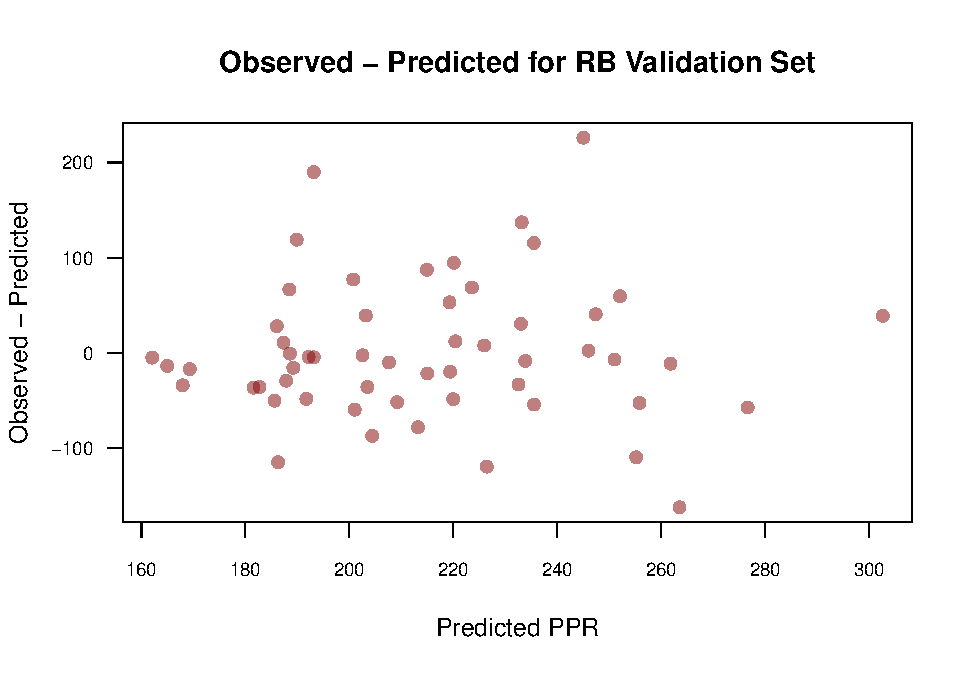
\includegraphics[width=0.85\linewidth]{stats_199_final_report_files/figure-latex/unnamed-chunk-7-1} \end{center}

There is not much of a trend in the residuals for the bagging model,
indicating that we should be alright to use it for predictions. With
this model, I looked at a variable importance plot with the percent
increase in MSE criterion to determine the most influential variables:

\begin{center}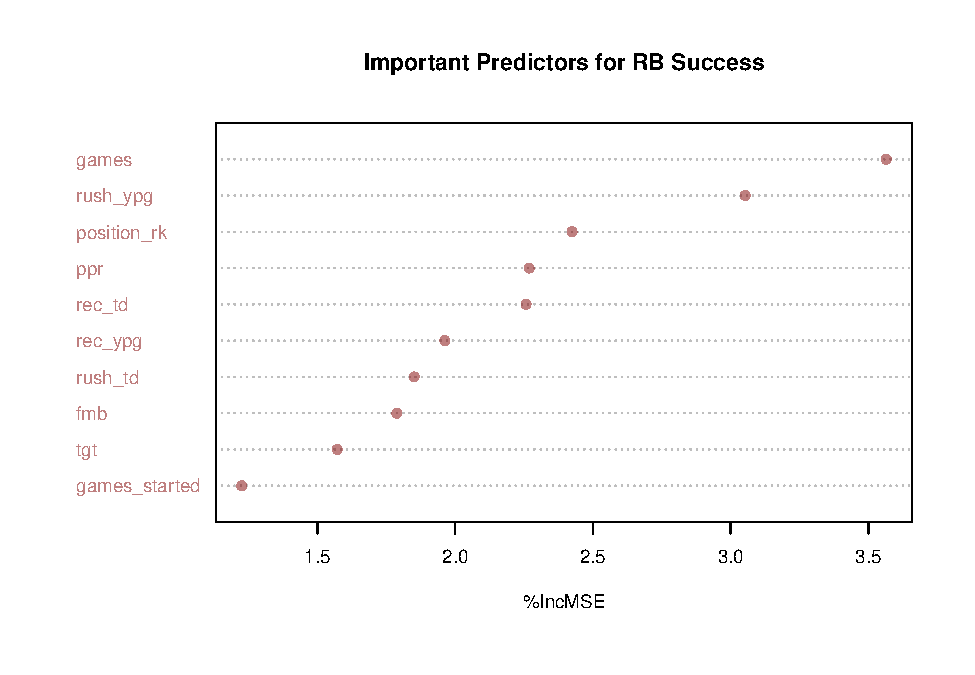
\includegraphics[width=0.85\linewidth]{stats_199_final_report_files/figure-latex/unnamed-chunk-8-1} \end{center}

From the above plot, it appears that the most influential feature is the
number of games played. This makes sense, as the more games a player
played, the better health he likely has, implying better performance in
the following season. We also see that rushing yards, like passing yards
for quarterbacks, have importance in determining success in the
following season. It is interesting to note that receiving touchdowns
carry more importance than rushing touchdowns. This reflects the
transition from a pure running back to an all-purpose back: in today's
NFL, running backs need to be versatile and adaptable--they need to be
able to catch the ball and play a role in the passing game in addition
to toting the rock.

Taking these factors into account, here are the predictions for next
season's running backs:

\begin{longtable}[]{@{}lr@{}}
\caption{RB Predictions for the 2021 NFL Season}\tabularnewline
\toprule
Player & Predictions \\
\midrule
\endfirsthead
\toprule
Player & Predictions \\
\midrule
\endhead
Nick Chubb & 258.0 \\
Dalvin Cook & 255.2 \\
Alvin Kamara & 237.5 \\
Aaron Jones & 235.2 \\
Chris Carson & 229.9 \\
David Montgomery & 223.4 \\
Austin Ekeler & 219.2 \\
Miles Sanders & 217.0 \\
David Johnson & 215.0 \\
Jonathan Taylor & 214.5 \\
\bottomrule
\end{longtable}

Again, it is interesting to note the absence of three running backs on
this list: Ezekiel Elliot, Saquon Barkley, and Christian McCaffrey. All
three running backs, who are elite in today's game by most measures,
suffered injury-plagued seasons, leaving my model unable to predict
their scores next season adequately. This list, though, does contain
new, up-and-coming running backs, potentially demonstrating the short
shelf life of running backs; running backs do not stay at an elite level
for a long time in the NFL.

\hypertarget{te}{%
\subsubsection{TE}\label{te}}

The tight end position ended up having a base model similar to that of
the quarterback: I chose the LASSO model, except without any
transformation to the response variable (MSE of 1219.308). While the
LASSO model post-transformation had a lower MSE (1204.194), I did not
find the difference drastic enough to warrant its usage; if two models
have a similar MSE, the simpler model is likely better (to avoid
overfitting). When considering a plot of predicted and observed values
from the validation data set, we see that the model appears to account
for most of the \emph{trend} in the data.

\begin{center}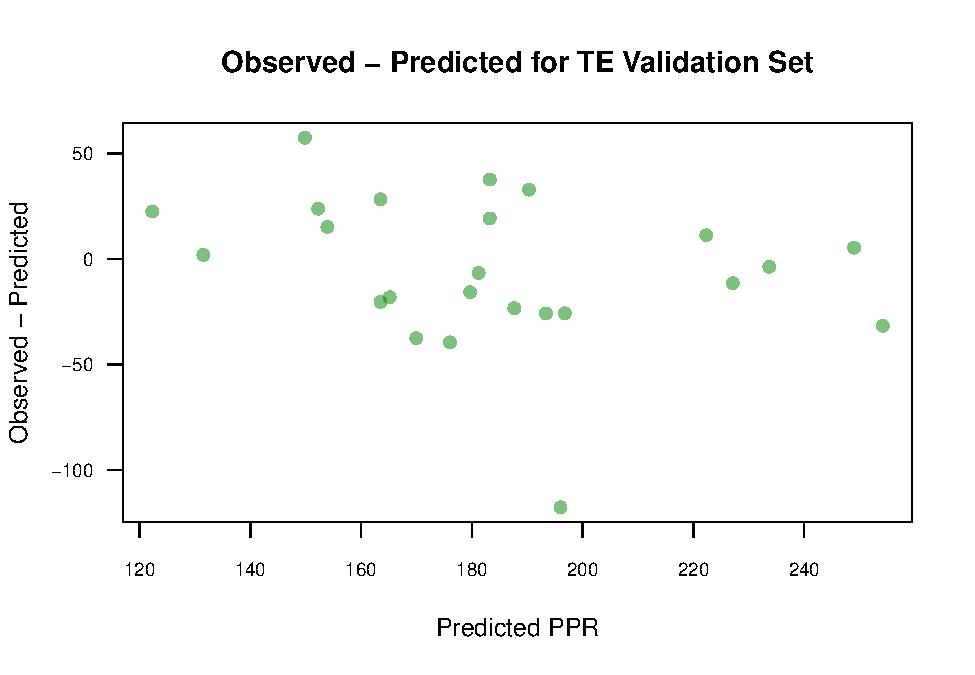
\includegraphics[width=0.85\linewidth]{stats_199_final_report_files/figure-latex/unnamed-chunk-10-1} \end{center}

However, there does appear to be one small issue with the LASSO model:
the outlier near the bottom of the plot, as I overpredicted fantasy
points by more than one hundred. When looking further into this
observation, I noticed that this observation is for Jordan Cameron of
the Cleveland Browns in 2013 and his subsequent disappointing 2014
season. In the 2014 season, Cameron was plagued by concussion injuries,
leaving him sidelined for multiple games and providing a reason for his
disappointing performance as depicted on the graph. Once again, my
model--nor any model I know--can predict injuries with a high success
rate, so this outlier is alright when predicting PPR points.

An interesting aspect of this model is its simplicity: for all the
various models I considered, the model created by LASSO simplified to a
univariate model: this time, though, the variable of choice was
receiving yards (instead of PPR, as was the case for my initial simple
linear model):

\[
\hat{y}= 0.1264(\text{receiving yards})
\]

Similar to the situation for the quarterback position, yardage totals
are a more reliable demonstration of a player's consistency than
touchdowns, so it makes sense that the model chose to emphasize that
statistic. Players with more receiving yards likely receive more targets
and receptions as well, placing themselves as volume options within a
given offense, as highlighted by the predictions for TEs next year:

\begin{longtable}[]{@{}lr@{}}
\caption{TE Predictions for the 2021 NFL Season}\tabularnewline
\toprule
Player & Predictions \\
\midrule
\endfirsthead
\toprule
Player & Predictions \\
\midrule
\endhead
Travis Kelce & 264.1 \\
Darren Waller & 223.2 \\
Mike Gesicki & 164.7 \\
T.J. Hockenson & 163.6 \\
George Kittle & 162.8 \\
Noah Fant & 162.7 \\
Mark Andrews & 161.2 \\
Logan Thomas & 154.4 \\
Rob Gronkowski & 154.1 \\
Hunter Henry & 153.9 \\
\bottomrule
\end{longtable}

The interesting part of these predictions occurs at slots \emph{(1)},
\emph{(2)}, and \emph{(5)}. Travis Kelce and Darren Waller are predicted
to \emph{massively} outclass their fellow tight ends, placing themselves
as a viable option for early-round picks (they appear to be
\emph{significantly better} than the rest of the pack). I also
highlighted George Kittle because Kittle missed \emph{a lot} of games
this season with injuries, yet is still predicted to be fifth (in the
middle of the pack). Intuitively, I think that had Kittle played a
complete season, his prediction for the 2021 NFL season would be on par
with Waller and Kelce, in a higher echelon than other tight ends.
Outside of the top 2 (and Kittle, had he played a full season), there
appears to be very little separating the tight ends from one another.

\hypertarget{wr}{%
\subsubsection{WR}\label{wr}}

Of the nine models I considered for the wide receiver position, the best
model was a ridge regression model after a response variable
transformation (i.e., transforming \(y\) into \(\log(y)\) before running
the ridge regression algorithm); it had the lowest MSE of all potential
candidate models (2279.374).

\begin{center}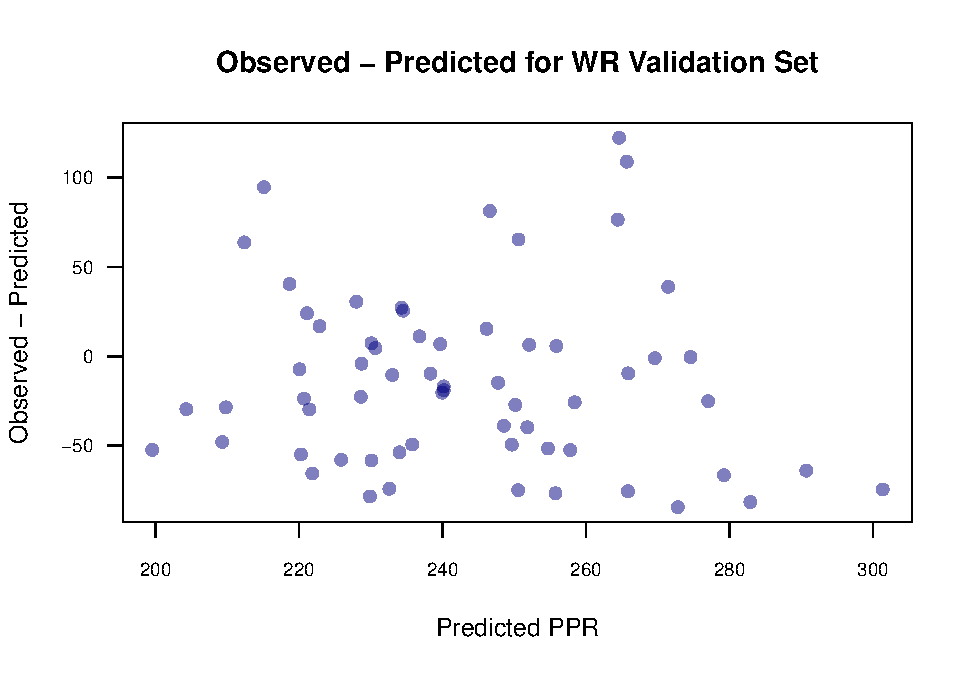
\includegraphics[width=0.85\linewidth]{stats_199_final_report_files/figure-latex/unnamed-chunk-13-1} \end{center}

The above plot shows that there appear to slight issues with the model.
It seems to underpredict values at the extreme ends, with increased
variability for the middle data points. However, these are slight
deviations, so on the whole the model seems justified for use.

This method--ridge regression--shrinks the coefficients of all included
predictors toward 0 similar to LASSO; however, unlike LASSO, it never
sets any predictors to exactly 0. This means that all predictors input
into the model initially will remain in the model after the best lambda
(\(\lambda\)) value is chosen; the relative size of each coefficient,
rather than just its presence, will denote the variable's importance.
Below, the coefficients may seem small; this is because of the log
transformation to the response. Regardless, at the moment we are more
interested in the relative value of these coefficients: larger
magnitudes indicate greater impact for a given variable, with positive
coefficients showing those variables had a positive relationship (i.e.,
an increase in these variables has a positive effect on the response),
while negative coefficients meant that as the value of that variable
increased, the response variable decreased.

\begin{longtable}[]{@{}lr@{}}
\caption{Top Coefficients for WR Predictions}\tabularnewline
\toprule
Statistic & Coefficient \\
\midrule
\endfirsthead
\toprule
Statistic & Coefficient \\
\midrule
\endhead
rec\_ypg & 0.0070 \\
yds\_per\_rush & 0.0038 \\
rec & 0.0021 \\
tgt & -0.0018 \\
age & -0.0017 \\
ppr & 0.0016 \\
games & -0.0016 \\
yds\_per\_rec & -0.0015 \\
games\_started & -0.0008 \\
rush\_att & 0.0005 \\
\bottomrule
\end{longtable}

\begin{center}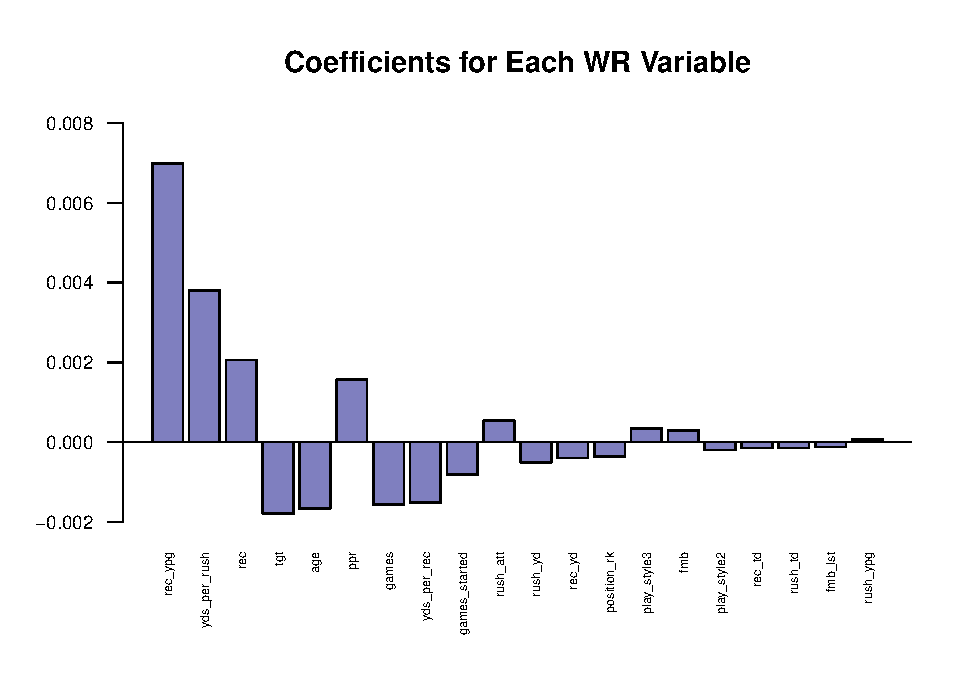
\includegraphics[width=0.85\linewidth]{stats_199_final_report_files/figure-latex/unnamed-chunk-14-1} \end{center}

\pagebreak

Of the six most influential variables, five seem to make sense,
regarding both size and sign. More receiving yards, receptions, and PPR
points tend to indicate higher levels of dependable future success,
while more targets and older age indicate a decrease in
production.\footnote{Targets and receptions are correlated, so if a
  player gets more receptions \emph{and} targets, there is a
  net-positive impact (since receptions have a greater impact). However,
  if a player has more targets but is unable to convert those targets
  into receptions, he will be seen as a less reliable player and thus
  less likely to succeed in the following season.} The one surprising
statistic that found its way into the mix was yards per rush attempt:
this statistic does not typically affect wide receivers, as they rarely
run the ball; this might indicate, though, a potential increase in the
usage of wide receivers in the offense through plays like the jet sweep.
However, this could also be the result of a confounding variable which I
have omitted in my analysis, as there might also be a link between how
often a wide receiver runs the ball and a third variable that explains
the increase in PPR scores.

\begin{longtable}[]{@{}lr@{}}
\caption{WR Predictions for the 2021 NFL Season}\tabularnewline
\toprule
Player & Predictions \\
\midrule
\endfirsthead
\toprule
Player & Predictions \\
\midrule
\endhead
Davante Adams & 318.8 \\
Stefon Diggs & 280.2 \\
Tyreek Hill & 273.5 \\
Will Fuller & 262.0 \\
Calvin Ridley & 259.0 \\
DeAndre Hopkins & 256.6 \\
A.J. Brown & 256.4 \\
Justin Jefferson & 256.0 \\
Chris Godwin & 252.3 \\
Adam Thielen & 248.8 \\
\bottomrule
\end{longtable}

For the wide receivers, there are no great surprises, as the players on
this list are young and valuable assets to their respective teams.
Similar to the running back position, there is the absence of two great
players--Julio Jones and Michael Thomas--who both struggled with
injuries during the 2020 season. Nonetheless, similar to the running
back predictions, many of the players on this top 10 list are young and
athletic players whose physical talents allow them to perform to their
full potential

\hypertarget{conclusion}{%
\subsection{Conclusion}\label{conclusion}}

After constructing the four primary models, I wanted to see how they
compared to one another. To do this, I decided to look at the difference
in what was considered ``the best MSE'' (i.e., the lowest MSE of the
possible models) for each model; I noticed that it varied by position.
The quarterback models hovered around 3000, running backs around 5500,
wide receivers around 2500, and tight ends around 1300. Intuitively,
this might indicate that the running back position is the ``least
predictable,'' but we have to consider the total variation present in
the data set (i.e., the mean squared deviations of the validation
set)\footnote{While the validation data set's mean squared deviations do
  vary by position, this variation is not statistically significant: in
  the earlier part, we failed to reject the null hypothesis that the
  variability for PPR scores was different for the positions.}.
Therefore, a better way to assess the ``strength'' of each model would
be to look at the models as a ratio with the mean squared deviations.

\begin{longtable}[]{@{}lr@{}}
\caption{Ratio of Model MSE to Mean Squared Deviations}\tabularnewline
\toprule
Position & Ratio \\
\midrule
\endfirsthead
\toprule
Position & Ratio \\
\midrule
\endhead
QB & 1.0353 \\
RB & 0.8156 \\
TE & 0.7299 \\
WR & 0.8546 \\
\bottomrule
\end{longtable}

When predicting the actual score for each quarterback next season, the
``best'' model performs \emph{worse} than if we simply predicted the
mean for each player (since the ratio is greater than 1). However, we
have to consider two things: \emph{(1)} we do not know next year's
average PPR scores--so that is a futile exercise--and \emph{(2)} the
goal of this analysis is not only to predict absolute predictions for
each player but also his performance \emph{relative to his peers}.
Therefore, if we simply predicted the mean for each player, we would be
unable to see which players would perform better than their counterparts
(and by how much).

Another thing to take into account is that the RB position, which had
the highest absolute validation MSE, was the second-best model regarding
relative MSE (after the tight end position). This shows us that, for our
validation data set, there tended to be more variability at the running
back position \emph{for the given set of players}\footnote{While the
  validation data set's mean squared deviations do vary by position,
  this variation is not statistically significant: in the earlier part,
  we failed to reject the null hypothesis that the variability for PPR
  scores was different for the positions.}, which is why we saw higher
MSE values at the running back position in the models.

Relative to the squared deviations of the validation set, we can see
that the tight end model performed best. One potential explanation would
be that the tight end position, in general, tends to be a ``high floor,
low ceiling'' position, which means that the players perform at a
relatively consistent level, but there isn't much
explosion/unpredictability when compared to the other three positions.

Again, while the ideal model minimizes the MSE, our main goal was to
predict the position of players relative to others at the same position;
therefore, predictions matter in that they show us how well a certain
player will perform relative to the others (i.e., a ranking). So, after
seeing the predictions for the four positions, we will construct the
``best lineup.'' We will ignore the flex position--it requires a
comparison between positions, which will be discussed below in the
``Further Analysis'' section--so the best lineup would include the top
QB, top two RB, two best WR, and best TE for a total of six players. In
addition to the starting lineup, I have included a backup of one player
for each position (which corresponds to the second-best QB and TE and
the third-best RB and WR).

\begin{longtable}[]{@{}lll@{}}
\caption{Best Potential Team}\tabularnewline
\toprule
Position & Starter & Backup \\
\midrule
\endfirsthead
\toprule
Position & Starter & Backup \\
\midrule
\endhead
QB & Josh Allen & Patrick Mahomes \\
RB1 & Nick Chubb & Alvin Kamara \\
RB2 & Dalvin Cook & \\
TE & Travis Kelce & Darren Waller \\
WR1 & Davante Adams & Tyreek Hill \\
WR2 & Stefon Diggs & \\
\bottomrule
\end{longtable}

The above table is an ideal scenario, as it is extremely unlikely--if
not impossible--for a manager in a twelve-team league to snag all of
these players. Instead, managers have to choose players based on who is
still available at the time of their pick.\footnote{This paper showed
  the top 10 predictions at each position. For a full list of
  predictions for next season for each position, see the GitHub
  repository (\url{https://github.com/ethan-allavarpu/stats-199}).}
Returning to a statement I made earlier in this paper, there are many
ways to prioritize a position. I prefer the method of the ``drop
off''--seeing which position has the largest difference between the top
two available players and drafting at that specified position--but this
is a subjective approach not backed by statistical analysis. One
statistically-supported claim I can make, though, is that the typical
strategy of prioritizing running backs and wide receivers solely because
they possess more variability than quarterbacks and tight ends is not
entirely founded in statistics; I have shown that the variability
present is statistically insignificant.

\newpage

\hypertarget{further-analysis}{%
\section{Further Analysis}\label{further-analysis}}

While I have performed a strong amount of analysis, there still exist
some gaps in my analysis that could, if implemented, demonstrate
improvement and expansion on a well-defined model.

In my predictive analysis, I considered a player's performance in the
prior season to predict his performance in the subsequent season. While
this style of analysis accounts for most of the variability, it does not
account for sustained performance over time. This issue becomes
prevalent when a strong player suffers an injury that leaves him
sidelined for most of (or the entirety of) the season (such as Christian
McCaffrey or Saquon Barkley during the 2020 NFL season), leaving little
to no data for the next season. However, intuition tells us that these
players would likely play well next season. In subsequent analyses, I
would consider some aspect of time-series analysis \emph{(1)} to account
for season-by-season improvement and \emph{(2)} to help lessen the
impact of an injury in a given season.

A player's performance is not only affected by injuries, but also by the
team for which that player plays. There are interactions between the
players on offensive-minded teams--for example, the Kansas City Chiefs
would have players that built on one another's successes--and switching
teams via free agency--a new player would have less chemistry with the
rest of the team and, in turn, less likely to perform at the same level
as he did on his former team.

Another instance in which predictions become impossible with my model is
for incoming rookies (first-year NFL players). These players may have
played exceptionally in college, but it is difficult to account for a
potential drop off in performance as a result of a new league as well as
stronger competition, which is why I based my predictions on prior
performance \emph{in the NFL}. Unfortunately, as a result of this
decision, I cannot predict the performance of rookies for the upcoming
seasons. To resolve this issue, one thing I may consider in the future
is to establish a separate model for first-year players that would be
based on their pre-NFL statistics, such as college performance and the
NFL Combine. However, I found this unsuitable for predicting fantasy
football success in general because I would have two separate
models--one for continuing players and another for rookies--which would
create conflicts when trying to merge predictions, which already was an
issue with my four separate models by position.

I could also attempt to combine all four positional models into a single
predictive method. By combining the models, I would be able to more
accurately assess the relationship between positions and predictions. In
its current state, my analysis establishes four models, providing a
ranking for each position, but the potential bias and variance differ
for each position--my model may overpredict for WR, but underpredict for
RB. Therefore, making comparisons between these two groups would be
inadequate, as simply combining the predictions would result in heavy
favoring of the wide receiver position in this hypothetical scenario.

The reason why I did not consider that approach for my research in this
paper is because I wanted to delineate between each position. I believe
that, inherently, the four groups were distinct enough that each would
be modeled best with an individual model. While I could have considered
a dummy variable for the position of each player, I feel as if it might
have been masked by the other variables present in the data set. I could
have also considered interactions between position and the other
variables, but it could have become complicated very quickly and likely
would have resulted in a similar model to the four individual models,
which would have the same result.

Lastly, there are a few positions that I did not consider in my analysis
which I might consider in follow-up analyses. There is the issue of the
flex position--a potential choice between RB, WR, and TE--which could be
solved if I found a way to combine the four individual models to predict
similar outcomes for each position. In its current state, my models seem
to favor the wide receiver position, which would indicate that managers
should look to select wide receivers to fill their flex position to
maximize the points they can get from a lineup.

There are also two other ``positions'' in a fantasy football lineup:
team defense (D/ST) and a kicker (K). I didn't consider these positions
because they have less of an impact on a manager's success than the four
core positions (and, as such, managers tend to choose these positions in
the last two-three rounds of a fantasy football draft). I could dive
deeper for another analysis, but I found it insignificant to the main
question I hoped to answer, so I omitted these positions for this paper.

\newpage

\hypertarget{links}{%
\subsection{Links}\label{links}}

\begin{itemize}
\tightlist
\item
  GitHub Repository: \url{https://github.com/ethan-allavarpu/stats-199}
\item
  Pro Football Reference:
  \url{https://www.pro-football-reference.com/years/2020/fantasy.htm}
\item
  ESPN: \url{https://www.espn.com}
\end{itemize}

\hypertarget{acknowledgments}{%
\subsection{Acknowledgments}\label{acknowledgments}}

\emph{I would like to acknowledge the help of Professor Michael Tsiang
and Professor Miles Chen in the development of the research discussed in
this paper and the paper itself. Professor Michael Tsiang helped guide
the process and provide help on how to consider various methods both for
modeling as well as defining success for this research. Professor Miles
Chen offered some tips on how to improve my model and potential
variables and interactions to consider for improved performance.}

\end{document}
